\section{Der Einfluss vom Codereview auf die Softwarequalität in den letzten Jahren}
\label{sec:Einfluss des Reviews}
Smartbear \cite{smartbear} führte im Jahr 2019 mit 1100 Softwareentwickler/Tester, IT- / Betriebsfachleute und Führungskräfte in 35 verschiedenen Branchen eine Umfrage durch. Die Teilnehmer der Umfrage arbeiten in Unternehmen mit unterschiedlichen Größen, von weniger als 25 Mitarbeitern bis zu über 10.000. Ähnliche Umfragen hat Smartbear regelmäßig durchgeführt.

Seit 2016 haben die Befragten identifiziert, dass der Codereview die beste Methode zur Verbesserung der Codequalität ist. Die Unit Testing im Jahr 2019 wurde als zweithöchste Wahl betrachtet und die Daten in der selben Rangliste vom Jahr 2019 zeigen: 25\% der Befragten wählen erneut den Codereview, was in der \cref{fig:Codereview-Softwarequalität} zu sehen ist.

\begin{figure}[H]
	\centering
	\includegraphics[width=1.0\textwidth]{Codereview-Softwarequalität}
	\caption[Einfluss der Codereview auf die Softwarequalität]{Codereview-Softwarequalität\\ \cite{smartbear}}
	\label{fig:Codereview-Softwarequalität}
\end{figure}

Die Wahrnehmung des Codereviews als Schlüssel für eine bessere Softwarequalität wurde durch die Daten vom Jahr 2019 bestätigt \cite{smartbear}.\unsure{soll das Zitat auch hier stehen ?}


\section{Zeit sparen oder im Review investieren}
\label{sec:reviewZeit}

Wie im \cref{sec:Einfluss des Reviews} erwähnt, dass Codereview und Softwarequalität eng verbunden sind, so dass es sich lohnt, die Zeit für den Review zu nehmen, um die Qualität des Quelltexts zu verbessern, zeigt auch die Umfrage von Smartbear welche sind die wichtigsten Vorteile, die der Review mit sich bringt. Zwar ist das Auffinden von Fehlern die Hauptmotivation, jedoch kann dieser Prozess dabei helfen, die Kommunikation des Teams zu verbessern, das Wissen zu übertragen und die Standardisierung zu erhöhen \cite{smartbear}. 

Die Folgende \cref{fig:Vorteile des Codereviews} stellt die Wichtigste Vorteile des Reviews dar.

\begin{figure}[H]
	\centering
	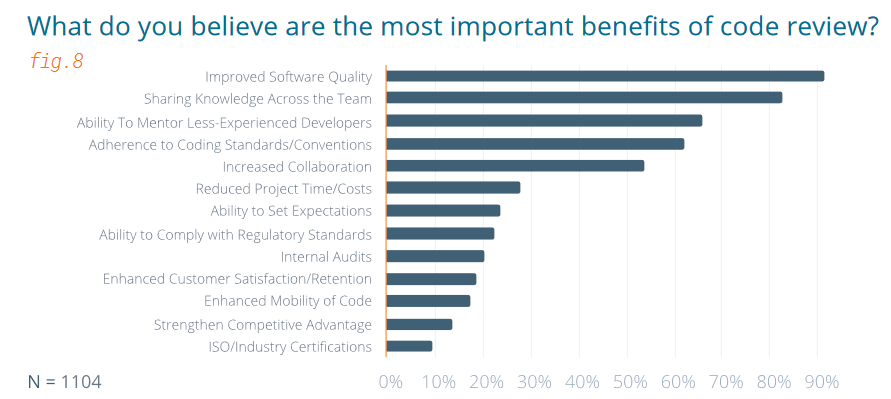
\includegraphics[width=1.0\textwidth]{Vorteile des Codereviews}
	\caption[Vorteile des Codereviews]{Die wichtigsten Vorteile des Codereviews\\ \cite{smartbear}}
	\label{fig:Vorteile des Codereviews}
\end{figure}

Die verbesserte Softwarequalität und die Wissensübertragung im gesamten Team sind seit 2015 die beiden wichtigsten Vorteile \cite{smartbear}.

\subsection{Wie oft soll der Programmierer für den Review Zeit nehmen ?}
\label{subsec:reviewerZeit}

Laut der Umfrage von Smartbear (Erklärung im \cref{sec:Einfluss des Reviews}) \cite{smartbear}, \textbf{67\%} der Befragten nehmen mindestens wöchentlich am Review teil, während \textbf{42\%} überprüfen den Code täglich.

\subsubsection{Die am häufigsten verwendete Methoden}
\label{subsubsec:Die am häufigsten verwendete Methoden}

Diese drei Methoden Ad-hoc, Meeting-basiert und Tool-basiert sind die gängigsten Ansätze zum Codereview (Die Erklärung dieser Methoden ist im \cref{subsec:Vorgehensmethoden} zu finden).
Die entsprechende Daten von der Smartbears Umfrage \cite{smartbear} dieser Methoden verdeutlicht das Balkendiagramm auf der \cref{fig:ReviewZeit} 

\begin{figure}[H]
	\centering
	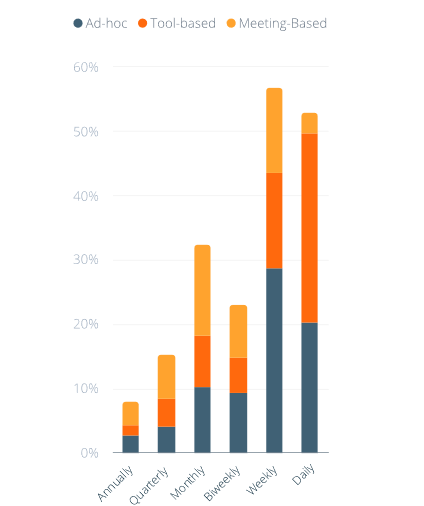
\includegraphics[width=0.7\textwidth]{ReviewZeit}
	\caption[Reviews Zeit]{Die benötigte Zeit für den Review\\ \cite{smartbear}}
	\label{fig:ReviewZeit}
\end{figure}

\begin{enumerate}
	\item \textbf{49\%} der Befragten führen mindestens wöchentlich den Review durch Ad-hoc oder Over-the-Shoulder durch, davon sind \textbf{20\%}, die ihr Code auf diese Weise 					täglich überprüfen.
	\item \textbf{44\%} der Befragten basiert ihren wöchentlichen Review auf Tools, davon sind \textbf{29\%}, die den Review mit Tools täglich machen.
	\item \textbf{16\%} der Befragten organisieren ein Meeting wöchentlich für den Review, davon sind \textbf{3\%}, die den Review auf diese Weise täglich durchführen.
\end{enumerate}


\section{Codereview-Tools}
\label{sec:Coderview-Tools}

\unsure{IDE Tools und  Static analysis tools erwähnen jeweils in subsec.}
\unsure{beschreibe was ist ein CRS und wie unterscheidet sich von andere Tools}
Es gibt 4 Bereiche, mit denen Entwickler ihre Code überprüfen.

\begin{itemize}
	\item \textbf{Repository-Verwaltungstools:} Diese Tools sind für die Verwaltung von Repositories zuständig. Entwickler können den Review durchführen, indem sie Pull-Anfrage an 				Teammitglieder senden oder auch durch andere Verfahren wie der Fall bei Helix Teamhub im \cref{subsec:HelixTeamHub}.
		Beispiele dafür sind z. B. :
		\begin{itemize}
			\item Bitbucket \cref{subsec:Bitbucket}
			\item Github \cref{subsec:Github}
		\end{itemize}
		
		Smartbears Umfrage zufolge verwenden \textbf{69\%} der Befragten Repository-Tools als Teil ihres Codereviews, unabhängig davon, ob sie den Review durch eine Pull-Anfrage 					durchführen oder in ein spezielles Peer-Codereview-Tool oder statisches Analysetool integrieren. Das bildet ein deutlicher Anstieg von \textbf{42\%} im Jahr 2018 							\cite{smartbear}.

	\item \textbf{IDEs:} Manche IDEs wie z. B Visual Studio\footnote{https://web.archive.org/web/20200507024443/https://visualstudio.microsoft.com/de/} bieten die Möglichkeit, direkt in 		der Umgebung den Review zu starten

	\item \textbf{Statische Analysetools:} Ein Beispiel dafür ist SonarQube\footnote{https://web.archive.org/web/20200508113558/https://www.sonarqube.org/}. Es ist eine Plattform, die 			automatisierte Regeln für die statische Code-Analyse definieren und benachrichtigt den Entwickler von seiner Pull-Anfrage, die durch Repository-Verwaltungstools erstellt wurden.

	\item \textbf{Peer-Codereview-Tools:} Beispiele sind: Crucible im \cref{subsec:Crucible} und Gerrit im \cref{subsec:Gerrit}. Das Hauptziel solcher Tools ist, einen einfachen und 				unkomplizierten Review anzubieten. Sie können kein Repository verwalten, haben aber andere Eingenschaften beispielsweise Änderungsvergleich anzeigen.
\end{itemize}

\subsection{Codereview-System}
\label{subsec:CRS}

Ein Codereview-System ist ein allgemeiner Begriff, der ein Tool beschreibt, das fähig ist, einen Codereview durchzuführen und diesen Review zu steuern. Dieses System kann ein Repository-Verwaltungstool, Statisches Analysetool, IDE oder ein Peer-Codereview-Tool sein, die im \cref{sec:Coderview-Tools} erläutert sind. Beispiele dafür sind im \cref{sec:CRS-Git}.

\section{Hauptziel}
\label{sec:Ziel}

Ziel dieser Arbeit: Ein \ac{CRS}, das gut für die Abteilung passt, aufbauen. Dieses System kann ein Repository-Verwaltungstool oder Peer-Codereview-Tool sein. Daher müssen ein paar Systeme Vorgestellt und miteinander nach bestimmten Kriterien verglichen werden. Außerdem sollen die ausgesuchte Systeme in der Abteilung getestet und ausgewertet werden.

\unsure{Reicht das? }

\subsection{Kriterien \& Erwartungen des Systems}
\label{sec:kriterien}

Folgende Eingenschaften sind die Kriterien, die in Betracht bei der Vorstellung von allen \acp{CRS} genommen werden sollen:

\begin{itemize}
	\item Es soll das \ac{VCS} Git unbedingt unterstützen
	\item Die Unterstützung vom \ac{VCS} \ac{SVN} ist vom Vorteil
	\item Es soll den Änderungsvergleich sowohl inline als auch Side-by-side deutlich darstellen können
	\item \ac{CI}/\ac{CD} Tools sollen in den Workflow eingebaut werden können oder in dem System integrieren sein
	\item Das System kann auf dem Eigenen Server hosten
	\item Hosten auf dem Server des Anbieters ist ein Vorteil
	\item Das System kann die Review-Kommentare nach Beenden des Reviews automatisch mit dem Haupt-Repository Zusammenführen
	\item Review-Kommentare sind auf Zeilenebene möglich
	\item Zugriffsverwaltung ist ein Vorteil
\end{itemize}
